% !TEX root = pfe-book2.tex
%!TEX TS-program = pdflatex
%!TEX encoding = UTF-8 Unicode


\cleardoublepage
%\mainmatter
\chapter{Solutions}
\label{ch-05}

\section{What a Solution Is}

If broth is salted and stirred with a spoon, no traces of salt will remain. It should not be thought that the grains of salt are simply not visible to the unaided eye. One will not succeed in detecting the tiny salt crystals in any way, because they have dissolved. If pepper is added to the broth, no solution will be obtained. One can even stir the broth for days on end, but the tiny black grains will not disappear.

But what do we mean when we say that a substance has dissolved? For the atoms or molecules composing it cannot vanish without a trace, can they? Of course not, and they do not vanish. When dissolving, only the grains of a sub­stance, crystals, accumulations of molecules of a single sort disappear. A \emph{dissolution} consists in stirring the particles a mixture in such a manner that the molecules of one substance are distributed between the molecules of another. A \emph{solution} is the mixture of molecules or atoms
of different substances.

A solution can contain various amounts of a solute.

The composition of a solution is characterized by its concentration, for example, the ratio of the number of grams of a solute to the number of litres of a solution.
As we add a solute, the concentration of a solution grows but not without bound. Sooner or later the solution will become saturated and will cease ``taking in'' the solute. The concentration of a saturated solution, i.e. the ``limiting'' concentration of the solution, is called the \emph{solubility}.

It is possible to dissolve a surprising amount of sugar in hot water. At a temperature of \SI{80}{\celsius}, a full glass of water will accept \SI{720}{\gram} of sugar with no residue. This saturated solution will be thick and viscous, and is called a sugar syrup by cooks. The figure we just gave for sugar is for a cup which holds \SI{0.2}{\liter}. Hence, the concentration of sugar in water at \SI{80}{\celsius} is equal to \SI{3600}{\gram\per\liter} (which is read ``grams per litre'').

The solubility of certain substances is highly dependent on the temperature. At room temperature (\SI{20}{\celsius}), the solubility of sugar in water falls to \SI{2000}{\gram\per\liter}. On the con­trary, the solubility of salt changes quite insignificantly with a change in temperature.

Sugar and salt dissolve well in water. But naphthalene is practically insoluble in water. Different substances dissolve quite differently in different solvents.

Solutions are used for growing monocrystals. If a small crystal of a solute is suspended in a saturated solution, then as the solvent evaporates, the solute will settle out on the surface of this crystal. Moreover, the molecules will preserve a strict order, and, as a result, the small crystal will be transformed into a large one, remaining a monocrystal.

\section{Solutions of Liquids and Gases}

Is it possible to dissolve a liquid in a liquid? Of course, it is. For example, vodka is a solution of alcohol in water (or, if you wish, of water in alcohol -- depending on what there is more of). Vodka is a real solution; the molecules of water and alcohol are completely mixed up in it.

However, such a result is not always obtained when two liquids are mixed.

Try adding kerosene to water. No matter how you stir, you will not succeed in obtaining a uniform solution; this is just as hopeless as trying to dissolve pepper in soup.

As soon as you stop stirring, the liquids arrange themselves in layers: the heavier water at the bottom, the lighter kerosene on the top. Kerosene with water and alcohol with water are systems having opposite properties with respect to their solubility.

However, there are also intermediate cases. If we mix ether with water, we shall clearly see two layers in the vessel. At first glance, it might appear that on the top is ether and at the bottom is water. But as a matter of fact, the lower and upper layers are solutions: at the bottom is water in which part of the ether is dissolved (the concentration being 25 grams of ether to a litre of water), while on the top is ether in which there is a noticeable amount of water (\SI{60}{\gram\per\liter}).

Let us now turn our attention to solutions of gases. It is clear that an unlimited amount of an arbitrary gas will dissolve in any other gas. Two gases always intermingle in such a way that the molecules of one penetrate between the molecules of the other. For gas molecules interact but slightly with each other, and so each gas behaves in the presence of another gas by, in a certain sense, not paying any ``attention'' to its cohabitant.

Gases can also dissolve in liquids. However, not in arbitrary amounts but in limited ones, not differing in this respect from solids. Moreover, different gases dis­solve differently, and these differences can be very great. Immense amounts of ammonia can dissolve in water (about 100 grams to half a glass of cold water), and large amounts of hydrogen sulphide and carbon dioxide. Oxygen and nitrogen are soluble in water in only negligible amounts (0.07 and 0.03 grams per litre of cold water).

Therefore, there is a total of only about one-hundredth of a gram of air in a litre of cold water. However, even this small amount plays a large role in life on the Earth, for fish breathe the oxygen of the air dissolved in water.

The greater the pressure of a gas, the more of it will be dissolved in a liquid. If the amount of a dissolved gas is not very great, there is a direct proportionality between it and the pressure of the gas above the surface of the liquid.

Who has not enjoyed a glass of cold soda, so good for quenching one's thirst. It is possible to obtain soda because of the dependence of the amount of a dissolved gas on the pressure. Carbon dioxide is driven into water under pressure (from the cylinders which are in every store where soda is sold). When soda is poured into a glass, the pres­sure falls to atmospheric and the water gives off the ``super­fluous'' gas in the form of bubbles.
Taking such effects into account, deep-sea divers should not rise rapidly from under the water to the surface. Addi­tional amounts of air dissolve in a diver’s blood under the high pressure of deep water. When rising, the pressure falls and air begins separating out in the form of bubbles which can stop up the blood vessels.

\section{Solid Solutions}

The word ``solution'' is applied to liquids in everyday life. However, there also exist solid mixtures whose atoms and molecules are uniformly distributed. But how can one obtain solid solutions? You won’t get them with the aid of mortar and pestle. Therefore, we must first turn the substances to be mixed into liquids, that is melt them, then mix the liquids and allow the mixture to solidify. One can also act otherwise, dissolving the two substances which we want to mix in some liquid and then evaporat­ing the solvent. Solid solutions might be obtained by such means. They might be, but they cannot ordinarily be so obtained. Solid solutions are rarities. If a piece of sugar is thrown into salty water, it will dissolve excel­lently. Evaporate the water; the minutest crystals of salt and sugar will be found at the bottom of the cup. Salt and sugar do not yield solid solutions.

It is possible to melt cadmium and bismuth in a single crucible. After cooling, we can see a mixture of cadmium and bismuth crystals through a microscope. Bismuth and cadmium do not form solid solutions either.

A necessary although not a sufficient condition for the emergence of solid solutions is the affinity of the molecules or atoms of the substances being mixed in form and dimensions. In this case, crystals of one sort are formed when the mixture freezes. The lattice points of each crystal are usually occupied randomly by atoms (molecules) of differ­ent sorts.

Alloys of metals of great technological value are fre­quently solid solutions. The dissolution of a small amount of an admixture can radically change the properties of a metal. A striking illustration of this is the obtaining of one of the most widespread materials in technology -- steel, which is a solid solution of small amounts of carbon (of the order of 0.5 of weight per cent, that is one atom of carbon to 40 atoms of iron) in iron, where the atoms of carbon are randomly distributed between the atoms of iron.

Only a small number of carbon atoms dissolve in iron. However, some solid solutions are formed by mixing substances in arbitrary proportions. Alloys of gold and copper can serve as an example. Crystals of gold and copper have lattices of the same type -- face-centred cubic. An alloy of copper with gold has the same lattice. An idea of the structure of alloys with an increasing percentage of copper can be obtained by conceptually deleting atoms of gold from the lattice and replacing them by atoms of copper. Moreover, the replacement occurs disorderly, with the copper atoms generally being distributed random­ly among the lattice points.

Alloys of copper with gold may be called solutions of replacement, whereas steel is a solution of a different type, a solution of introduction.

In the vast majority of cases, solid solutions do not arise, and, as has been said above, after cooling we can see in the microscope that the substance consists of a mixture of tiny crystals of both substances.

\section{How Solutions Freeze}

If a solution of any salt in water is cooled, it will be discovered that the freezing point has been lowered. Zero mark is past, but solidification does not occur. Only at a temperature of several degrees below zero do tiny crystals appear in the liquid. They are tiny crystals of pure ice: salt does not dissolve in solid ice.

The freezing point depends on the concentration of a solution. Increasing the concentration of a solution, we shall lower its freezing point. A saturated solution has the lowest freezing point. The decrease in the freezing point of a solution is not at all small: thus, the saturated solu­tion of sodium chloride in water freezes at \SI{-21}{\celsius}. With the aid of other salts, we can achieve an even greater fall in temperature; calcium chloride, for example, enables us to bring the freezing point of a solution down to \SI{-5}{\celsius}.

Let us now consider how the process of freezing takes place. After the first tiny crystals of ice have fallen out of a solution, the concentration of the solution increases. Now the relative number of alien molecules grows, the obstacles to the process of the crystallization of water also increase and the freezing point falls. If we do not further lower the temperature, then crystallization will cease. With a further lowering of temperature, tiny crys­tals of water (the solvent) continue separating out. Finally, the solution becomes saturated. A further enrich­ment of the solution by the solute becomes impossible, and the solution solidifies at once; moreover, if we look at the frozen mixture through a microscope, we can see that it consists of tiny crystals of ice and tiny crystals of salt.

Consequently, the freezing of a solution is unlike that of a simple liquid. The process of freezing is spread out over a wide temperature interval.

What will happen if we pour salt on some frozen surface? The answer to this question is well known to yard men -- as soon as salt comes in contact with ice, the ice begins melting. In order that this phenomenon take place, it is necessary, of course, that the freezing point of a saturated salt solution be lower than the temperature of the air. If this condition is met, the mixture of ice and salt is in an alien phase region, namely, in the region of stable exi­stence. Therefore, the mixture of ice with salt will turn into a solution, i.e. the ice will melt and the salt will dissolve in the water so formed. Finally, either all the ice will melt or else a solution of such a concentration will be formed that its freezing point will be equal to the tem­perature of the surroundings.

Suppose that a yard whose area is \SI{100}{\meter\squared} is covered by a \SI{1}{\centi\meter} layer of ice -- this is quite a bit of ice, about one ton. Let us calculate how much salt is needed to melt this ice if the temperature is \SI{-3}{\celsius}. For such a freezing (melting) point the concentration of a salt solution must be \SI{45}{\gram\per\liter}. Approximately one litre of water corresponds to one kilogram of ice. Hence, in order to melt one ton of ice at \SI{-3}{\celsius}, 45 kg of salt are needed. A much smaller amount is used in practice since one does not seek the complete melting of all the ice.

Ice melts when mixed with salt, and salt dissolves in water. But heat is required for melting, and the ice takes it from its surroundings. Therefore, the addition of salt to ice leads to a decrease in temperature.

We are now in the habit of buying ice cream, but it was previously made at home. In this connection, a mixture of ice and salt played the role of a coolant.

\section{Boiling of Solutions}

Boiling of solutions has a lot in common with their freezing.

The presence of a solute hinders crystallization. For the very same reasons, a solute also hinders boiling. In both cases it is as though alien molecules were fighting to retain a solution which is as diluted as possible. In other words, the alien molecules stabilize the state of the basic substance (i.e. facilitate its existence), which can dissolve them.

Therefore, alien molecules impede the crystallization of a liquid, and so lower the freezing point. In exactly the same way, alien molecules impede the boiling of a liquid, and so raise its boiling point.

It is curious that within certain limits of concentration (for not very concentrated solutions), neither the lowering of the freezing point of a solution nor the raising of its boiling point depends in the least on the properties of the solute but is determined only by the number of its molecules. This interesting circumstance is used for the determination of the molecular mass of soluble substances. This is done with the aid of a remarkable formula (we cannot give it here), which relates the change in the freez­ing or boiling point to the number of molecules in a unit volume of a solution (and to the heat of fusion or boiling).

The boiling point of water is raised one-third as much as its freezing point is lowered. Thus, sea water containing approximately 3.5\% of salt has a boiling point of \SI{100.6}{\celsius}, while its freezing point is lowered by \SI{2}{\celsius}.

If one liquid boils at a higher temperature than another, then (at the same temperature) its vapour pressure is lower. Hence, the vapour pressure of a solution is less than that of the pure solvent. One can judge the differ­ence on the basis of the following values: the vapour pres­sure at \SI{20}{\celsius} equals \SI{17.5}{\milli\meter\mercury} and the vapour pressure of a saturated solution of sodium chloride at the same temperature is \SI{13.2}{\milli\meter\mercury}.

Vapour with a pressure of \SI{15}{\milli\meter\mercury}, unsaturated for water, will be supersaturated for a saturated salt solu­tion. In the presence of such a solution, the vapour starts condensing and uniting with the solution. Of course, not only a salt solution but also powdered salt will take wa­ter vapour out of the air. In fact, the very first drop of water falling on the salt will dissolve it and create a saturated solution.

The absorption of water vapour from the air by salt leads to the salt’s becoming moist. This is well known to hosts and affords them grief. But this decrease in vapour pressure over a solution can also be of benefit: it is used for drying air in laboratory practice. Air is passed through calcium chloride, which is the record holder in taking moisture out of the air. While a saturated solution of sodium chloride has a vapour pressure of \SI{13.2}{\milli\meter\mercury}, that of calcium chloride is \SI{5.6}{\milli\meter\mercury}. The vapour pres­sure will fall to this value when it is passed through a sufficient amount of calcium chloride (\SI{1}{\kilo\gram} of which “has room for” approximately \SI{1}{\kilo\gram} of water). This is a negligible humidity, and such air may be regarded as dry.

\section{How Liquids Are Freed of Admixtures}

Distillation is one of the most important means of freeing liquids of admixtures. The liquid is boiled and the vapour is sent into a refrigerator. When cooled, the vapour turns into a liquid once more, but this liquid will be purer than the initial one.
It is easy to get rid of solids dissolved in a liquid with the aid of distillation. Molecules of such substances are practically absent in water vapour. Distilled water is obtained in this way -- completely tasteless pure water devoid of mineral admixtures.

However, using evaporation, we can also get rid of liquid admixtures and separate a mixture consisting of two or more liquids. In this connection, we make use of the fact that two liquids forming a mixture do not boil with the same ``ease''.

Let us see how a mixture of two liquids, for example, of water and ethyl alcohol, taken in equal amounts (100 proof vodka), will behave when boiled.

Under standard pressure, water boils at \SI{100}{\celsius} and al­cohol at \SI{78}{\celsius}. The mixture we are dealing with will boil at the intermediate temperature of \SI{81.2}{\celsius}. Alcohol boils more easily, so its vapour pressure is greater, and for an initial fifty-per cent composition of the mixture, the first portion of vapour will contain 80\% alcohol.

We can draw off the portion of vapour so obtained into a refrigerator and obtain a liquid enriched by alcohol. This process can be further repeated. However, it is clear that such a method is not practical, for with each suc­cessive distillation less and less substance will be obtained. In order that there be no such loss, so-called fraction­ating (i.e. purifying) columns are applied for the pur­pose of cleaning a liquid.

The idea behind the structure of this interesting appa­ratus consists in the following. Imagine a vertical column whose lower part contains a liquid mixture. Heat is supplied below the column and cooling is carried out above it. The vapour formed by boiling rises to the top and condenses; the resulting liquid flows down. For a fixed heat supply from below and heat removal from above, the countercurrents of vapour, going up, and liquid, flowing down, are established in the closed column.

Let us fix our attention on some horizontal cross-section of the column. The liquid passes downwards, and the vapour upwards, through this cross-section; moreover, none of the substances composing the liquid mixture stays behind. If we are dealing with a column containing a mixture of alcohol and water, the amount of alcohol passing upwards and downwards, just as the amount of water passing upwards and downwards, will be equal. Since the liquid is going down and the vapour is coming up, this means that the compositions of the liquid and of the vapour are identical at any height in the column.

As has been just explained, the equilibrium of the liquid and the vapour of a mixture of two substances requires, on the contrary, a difference between the composi­tions of these phases. Therefore, the conversion of liquid into vapour, and of vapour into liquid, takes place at any height in the column. Moreover, the high-boiling compo­nent condenses and the low-boiling component passes from the liquid to the vapour.

Consequently, it is as though the rising vapour were taking away the low-boiling component and the down­ flowing liquid were continually being enriched by the high-boiling component. The composition of the mixture will become different at each height: the higher the mixture, the greater the percentage of the low-boiling com­ponent. In the ideal case, a pure layer of the low-boiling component will be on the top and a pure layer of the high- boiling component will be at the bottom.

The substances should now be drawn off, only as slowly as possible, in order that the ideal picture just outlined not be disturbed, the low-boiling one from the top, and the high-boiling one from the bottom.

In order to carry out the separation, or rectification, in practice, we must make it possible for the counter-cur­rents of liquid and vapour to thoroughly mix. To this end, the currents of liquid and vapour are delayed with the aid of plates distributed one above the other and connected by means of overflow pipes. The liquid can flow down to a lower level from an overfilled plate. The rising vapour (0.3-1\si{\meter\per\second}) forces its way through a thin layer of liquid. The diagram of a column is shown in \figr{fig-5.1}.

\begin{figure}[!ht]
\centering
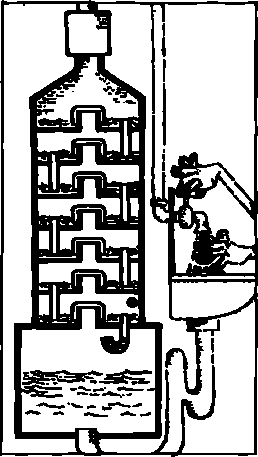
\includegraphics[width=0.5\textwidth]{figures/fig-05-01.pdf}
\caption{Separating liquids using distillation.}
\label{fig-5.1}
\end{figure}

One does not always succeed in purifying a liquid com­pletely. Certain mixtures possess an ``unpleasant'' prop­erty: for a definite composition, the ratio of the compo­nents of the evaporating molecules is the same as that in the liquid mixture. In this case, of course, a further pu­rification by means of the method described becomes im­possible. Such is the mixture containing 96\% alcohol and 4\% water: it yields a vapour of the same composition. Consequently, 96\% alcohol is the best that can be ob­tained by the evaporation method.

Rectification (or distillation) of liquids is an important process in chemical technology. For example, gasoline is obtained from oil with the aid of rectification.

It is a curious fact that rectification is the cheapest method of obtaining oxygen. For this, of course, one must change air to the liquid phase beforehand, after which one can separate it into almost pure nitrogen and oxygen by means of rectification.

\section{Purification of Solids}

On a phial containing a chemical substance alongside of the chemical name one can see, as a rule, the following notation: ``pure'', ``pure for analysis'' or ``spectroscopically pure''. They are used to mark the degree of purity of a substance: ``pure'' means a rather slight degree of purity -- there may possibly be an admixture of the order of 1\% in the substance; ``pure for analysis'' means that admixtures constitute not more than several tenths of a percent of the substance; ``spectroscopically pure'' is not easy to obtain, since spectral analysis detects an admixture of several thousandths of a percent. The inscription ``spectroscopically pure'' permits us to be confident that the purity of the substance is characterized by at least ``four nines'', i.e. that the content of the basic substance is not less than 99.99\%.

The need for pure solids is quite great. Admixtures of several thousandths of a percent can change many phys­ical properties, and in one special problem of exception­al interest to modern technology, namely the problem of obtaining semiconductors, technologists require a purity of seven nines. This means that one unnecessary atom among ten million necessary ones prevents us from solv­ing engineering problems! We take recourse in special methods for obtaining such ultrapure materials.

Ultrapure germanium and silicon (these are the main representatives of semiconductors) can be obtained by slowly drawing out a growing crystal from a melt. A rod on whose tip a seed crystal is attached is brought to the surface of melted silicon (or germanium). We then begin slowly raising the rod; the crystal coming out of the melt is made up of the atoms of the basic substance, while the atoms of the admixture remain in the melt.

The method of so-called zone refining has been applied more widely. A rod of arbitrary length and several mil­limetres in diameter is made out of the material being purified. A small cylindrical oven is placed alongside the rod enveloping it. The temperature in the oven is high enough for melting, and the part of the metal which is inside the oven melts. Therefore, a small zone of melted metal moves along the rod.

The atoms of an admixture usually dissolve much more easily in a liquid than in a solid. Consequently, at the boundary of the melted zone, the atoms of admixture pass from solid parts to the melted zone and do not pass back. It is as though the moving melted zone were dragging off the atoms of the admixture together with the melt. The oven is turned off during the reverse motion, and the operation of pulling the melted zone past the rod of metal is repeated many times. After a sufficient number of cycles, it only remains to saw off the polluted end of the rod. Ultrapure materials are obtained in a vacuum or in an atmosphere of inert gas.

When there is a large fraction of alien atoms, purifi­cation is carried out by other methods, the zone melting and pulling a crystal out of a melt being applied only for the final purification of the material.

\section{Adsorption}

Gases rarely dissolve in solids, i.e. rarely penetrate crystals. But there exists a different kind of absorption of gases by solids.  Molecules of a gas accumulate on the surface of a solid body -- this peculiar adherence is called \emph{adsorption}.\footnote{Adsorption should not be confused with absorption, which simply means taking in.} Thus, adsorption occurs when molecules cannot penetrate within a body, but successfully stick to its surface.

To be adsorbed means to be absorbed by a surface. But can such a phenomenon really play a significant role? In fact, a layer one molecule thick, even on a very large object, will weigh a negligible fraction of a gram.

Let us perform the appropriate calculations. The area of a small molecule is about \SI{10}{\angstrom\squared}, i.e. \SI{d-15}{\centi\meter\squared}. Hence, \num{d15} molecules will fit into a square centimetre. That many molecules, say, of water, do not weigh much: \SI{3d-8}{\gram}. Even in a square metre, there will be room for only \SI{0.0003}{\gram} of water.

More noticeable amounts of a substance will form on surface areas of hundreds of square metres. There is as much as \SI{0.03}{\gram} of water (\num{d21} molecules) per \SI{100}{\meter\squared}.

But do we come across such sizable surface areas in our laboratory practice? However, it is not hard to grasp that sometimes very small bodies, fitting onto the tip of a teaspoon, have enormous areas of hundreds of square metres.

A cube whose edges are \SI{1}{\centi\meter} long has a surface area of \SI{6}{\centi\meter\squared}. Let us cut such a cube into 8 equal cubes with \SI{0.5}{\centi\meter} edges. The small cubes have faces with an area of \SI{0.25}{\centi\meter\squared}. There are $6 \times 8 = 48$ such faces in all. Their total area is equal to \SI{12}{\centi\meter\squared}. The surface area has been doubled.

Thus, every splitting of a body increases its surface. Let us now break up a cube with a 1-cm side into small chips one micrometre long: $\SI{1}{\micro\meter} = \SI{d-4}{\centi\meter}$, so the large cube will be divided into \num{d12} pieces. Each piece (let us assume for the sake of simplicity that it, too, is cubic) has a surface area of \SI{12}{\micro\meter\squared}, i.e. \SI{6d-8}{\centi\meter\squared}. The total surface area of the chips is equal to \SI{6d4}{\centi\meter\squared}, i.e. \SI{6}{\meter\squared}. And such a splitting is by no means the limit.

It is quite understandable that the specific surface area (i.e. the surface area of one gram of a substance) can be immense. It grows rapidly with the crushing of a sub­stance -- for the surface area of a grain decreases in proportion to the square of its linear dimension, and the number of grains in a unit of volume increases in proportion to the cube of this dimension. A gram of water poured onto the bottom of a glass has a surface area of several square centimetres. The same gram of water in the form of raindrops has a surface area of about tens of square centimetres. But one gram of droplets of fog has a surface area of several hundred square metres.

If you break up a piece of coal (the finer the better), it will be capable of adsorbing ammonia, carbon dioxide and many toxic gases. This last property has assured for coal an application in gas-masks. Coal breaks up partic­ularly well, and the linear dimensions of its particles can be reduced to ten angstroms. Therefore, one gram of special coal has a surface area of several hundred square metres. A gas-mask with coal is capable of absorbing tens of litres of gas.

Adsorption is widely employed in the chemical indus­try. Molecules of different gases adsorbed on a surface come in close contact with each other and participate in chemical reactions more easily. In order to speed up chemical processes, one frequently makes use of finely split-up metals (nickel, copper and others) as well as of coal. Substances increasing the rate of a chemical reac­tion are called catalysts.

\section{Osmosis}

Among the living tissues, there are peculiar membranes which have the ability of letting water molecules pass through them, remaining impermeable to molecules of substances dissolved in water. The properties of these membranes are the causes of physical phenomena bearing the name ``osmotic'' (or simply ``osmosis'').

Imagine that such a semipermeable partition divides a pipe made in the form of the letter $U$ into two parts. A solution is poured into one of the elbows of the pipe, and water or some other solvent into the other elbow. Having poured the same amount of liquid into both elbows, we shall discover with surprise that there is no equilibrium when the levels are equal. After a short time, the liquids settle down at different levels. Moreover, the level is raised in the elbow containing the solution. The water separated from the solution by the semipermeable par­tition tends to dilute the solution. It is just this phenom­enon that bears the name \emph{osmosis}, and the difference in height is called the \emph{osmotic pressure}.

\begin{figure}[!ht]
\centering
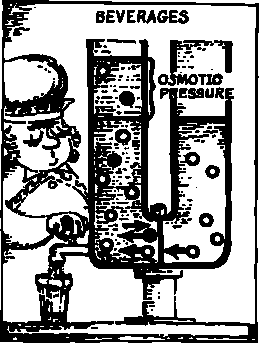
\includegraphics[width=0.5\textwidth]{figures/fig-05-02.pdf}
\caption{Osmotic pressure and beverages.}
\label{fig-5.2}
\end{figure}
But what is the cause giving rise to osmotic pressure? In the right-hand elbow of the vessel (\figr{fig-5.2}), pres­sure is exerted only by water. In the left-hand elbow, the total pressure is the sum of the pressure of the water and that of the solute. But the door is open only for the water, and equilibrium in the presence of the semipermeable partition is established not when the pressure from the left equals the total pressure from the right, but when the pressure of the pure water is equal to the “water” portion of the pressure of the solution. The arising difference between the total pressures us equal to the pressure of the solute.

This excess of pressure is precisely the osmotic pres­sure. As experiments and computations show, the osmotic pressure is equal to the pressure exerted by a gas composed of the solute and occupying the same volume. It is therefore not surprising that osmotic pressure is measured in impressive numbers. The osmotic pressure arising in one litre of water when it dissolves 20 grams of sugar would balance a column of water \SI{14}{\meter} in height. 

Running the risk of arousing unpleasant memories in the reader, we shall now examine how the laxative ac­tion of certain salt solutions is related to osmotic pres­sure. The walls of the intestines are semipermeable to a number of solutions. If a salt does not pass through the walls of the intestines (this is true of Glauber’s salt), then in the intestines there arises an osmotic pressure and this pressure ``sucks'' water through the tissues from the
organism into the intestines.

Why does very salty water fail to quench one’s thirst?

It turns out that osmotic pressure is guilty of this, too. The kidneys cannot eliminate urine with the osmotic pressure greater than the pressure in the tissues of the organism. Consequently, an organism which has acquired salty sea water does not only fail to give it to the tis­sue liquids, but, on the contrary, eliminates water taken away from the tissues along with urine.